\documentclass[a4paper, 12pt]{article}

\usepackage[utf8]{inputenc}
\usepackage{amsmath}
\newcommand{\norm}[1]{\left\lVert#1\right\rVert}

\usepackage[]{amsfonts}
\usepackage[]{graphicx}
\usepackage{wrapfig}
\graphicspath{{figures/}}

\title{CS231A Course Notes 6b: Feature Descriptors}
\author{Sahaj Garg and Marcus Gomez}
\date{}

\renewcommand\emph{\textbf}

\numberwithin{equation}{section}
\begin{document}

\maketitle

\section{Introduction}
In the previous part of this course notes, we discussed feature detectors. Now, we discuss how to compute descriptors to characterize our previously detected features. 

\section{Descriptors}
By describing features, we can eventually match keypoints and use them for tasks such as estimation, matching, indexing, and detection/recognition. We begin by motivating properties of good descriptors, then consider a series of examples, their advantages, and disadvantages . 

\subsection{Properties of Good Descriptors}
Useful feature detectors will maintain a number of properties. First, they should be invariant to changes in illumination, pose, scale, and intraclass variability across images. Otherwise, they will not be able to similarly describe similar features across images. Second, they should be highly distinctive. Intuitively, we want different features/keypoints to have very different descriptors so that the descriptors have high discriminative power.  

\subsection{Normalized Correlation}
The simplest feature detector would involve unrolling pixel values of a size $M \times N$ blob into a $MN$ dimensional vector. However, as is, this will not be invariant to changes in illumination and intensity. So, we can normalize the feature vector w for any given image:

$$ w_n = \frac{w - \bar{w}}{\norm{w - \bar{w}}}$$

This transformation makes the descriptor invariant with respect to affine transformation of the illumination condition. For example, if a second image's pixel values are all scaled by a, and increased by b (for example, in a change of illumination), this normalization will remove the changes. It will overall make the patches have zero mean (by the translation $\bar{w}$) and have unit variance (by dividing by the norm).  

Detection of this descriptor in another image can be performed using the \textbf{normalized correlation}. In this procedure, one slides a window over the second image, and computes the correlation $w_n \cdot w_n'$ for every window, and claims the detected region to be the location of maximum cross correlation.  

$$ w_n \cdot w_n' = \frac{(w - \bar{w})(w' - \bar{w'})}{\norm{w - \bar{w}}\norm{w' - \bar{w'}}}$$

\begin{figure}
\centering
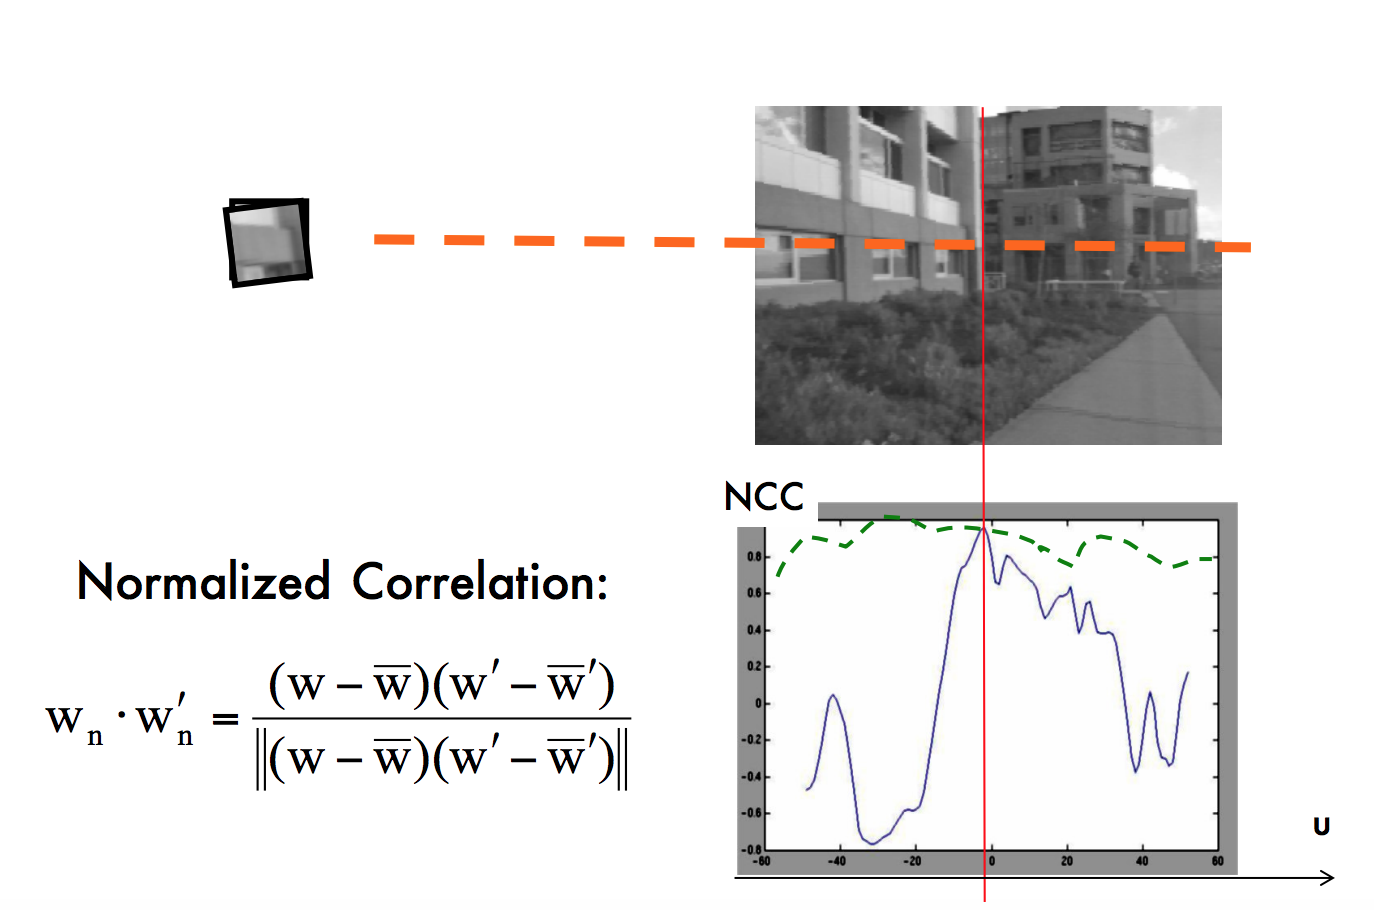
\includegraphics[width=0.7\textwidth]{ncc}
\caption{Issues that arise for slight changes in pose for a keypoint in the normalized cross correlation. Slightly changing the pose changes the normalized correlation response from having a peak at the correct location (black) to noise (green dash).}
\end{figure}

Unfortunately, this method isn't sufficient to satisfy all the properties we desired; specifically, it is sensitive to small changes in location, pose, scale, intra-class variability, and is poorly distinctive. For example, if the pose is slightly changed, the values of the normalized cross correlation are dramatically different and the maximum is not meaningful. 

One small adjustment to slightly improve the patch feature descriptor is to use a \textbf{bank of filters}. In this procedure, a window is convolved with a set of filters, and the descriptor is the concatenation of the unrolled representations of each convolved window. Overall, this is more robust than the patch descriptor, but is still sensitive to pose variations. 

\begin{figure}[h]
\centering
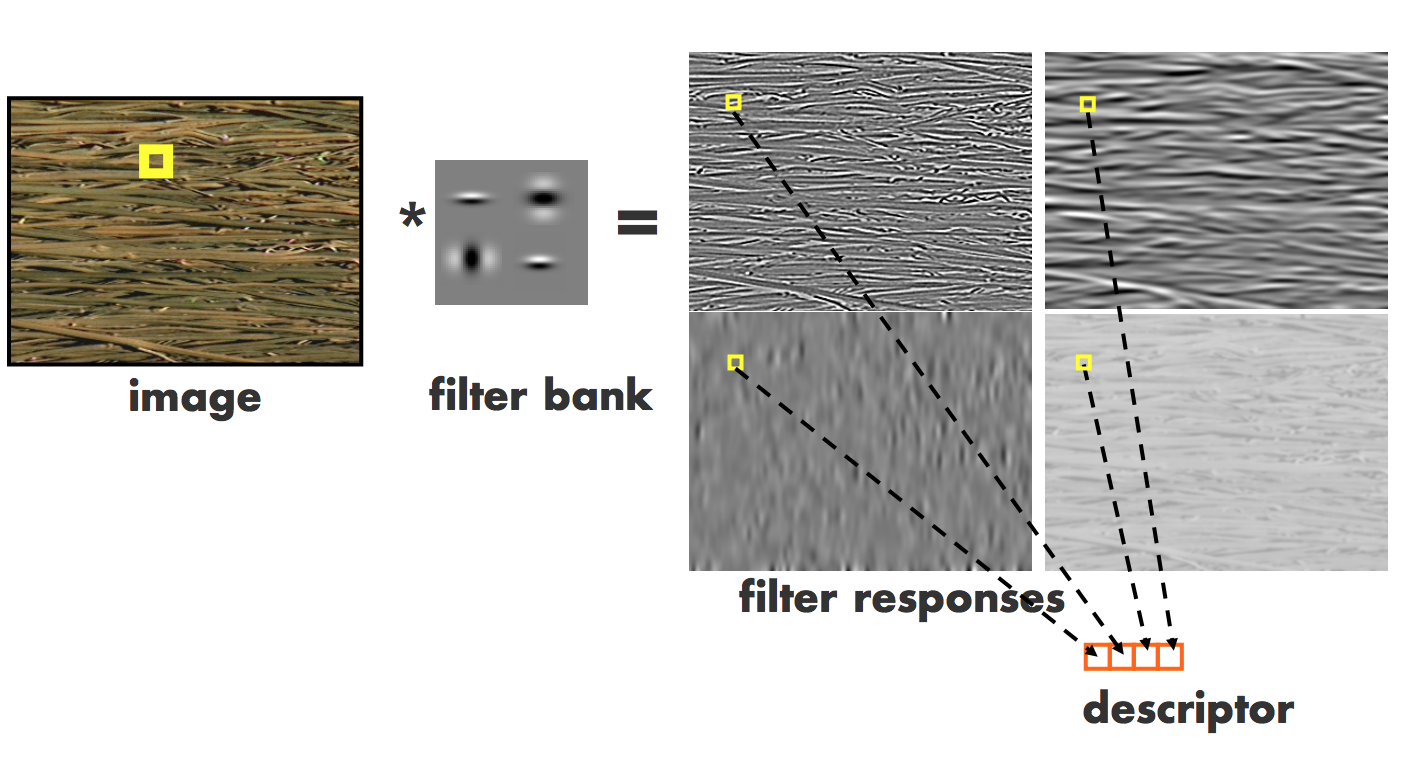
\includegraphics[width=0.7\textwidth]{filter_bank}
\caption{Using a bank of filters is slightly more robust.}
\end{figure}


\subsection{SIFT}
SIFT, or the Scale Invariant Feature Transform, is a highly effective descriptor uses gradients of changes in pixel intensity to describe keypoints. We describe the SIFT method for detecting keypoints, then the method for describing them.

\subsubsection{Detecting Keypoints}
First, keypoints and their associated scales are detected using Difference of Gaussians (DoG) described above. Some keypoints are rejected if they do not pass a minimum contrast threshold or if they correspond to edges. Edge correspondence is measured by considering the Hessian at a pixel, and comparing $\frac{Tr(H)^2}{Det(H)}$ to a threshold. (Brief intuition: the trace is the sum of the eigenvalues, and the determinant is the product of the eigenvalues. For edges, one of the eigenvalues will be close to zero, so this ratio will be large. Filtering for keypoints that have a ratio smaller than a threshold will yield only corners/blobs of interest). 

\subsubsection{Rotational Invariance}
Once keypoints have been detected, we seek to find a way to make them rotationally invariant. The intuition behind this step is to realize that if a keypoint is rotated, we expect that the dominant orientation of the gradients is rotated the same way. As a result, if we can find the dominant orientation, we can re-orient the keypoint by this direction. In order to do this, we compute the gradients of all pixels in the feature and weight it by a Gaussian centered at the center of the keypoint (with scale $\sigma$ = 1.5 times the scale of the keypoint). We then compute a histogram of these gradients, with 36 bins corresponding to orientations and values based on the weighted magnitudes of the gradients. We might intuitively take the orientation that has the maximum value in the histogram. In order to make the algorithm more stable, though, SIFT chooses any peak within 80\% of the highest peak, which creates multiple keypoints for ~15\% of keypoints. The orientation is stored, the feature is reoriented by the dominant orientation, and then the feature descriptor is computed using the below procedure: 

\subsubsection{Computing SIFT Descriptor}
The overall procedure is based on computing histograms of gradients throughout the image.

\begin{enumerate}
\item Divide the image into $N \times N$ spatial bins.
\item Divide each spatial bin into smaller subsections (typically, a 4x4 grid within each bin), and for each of these, compute the gradient in the segment. This can be done through a finite differences approach, or using the Sobel kernel from earlier in this notes. 
\item For each spatial bin $i$, compute a histogram $h_i$ of the gradients in the bin with M orientation categories. This constructs a M-dimensional vector. 

\begin{figure}[h]
\centering
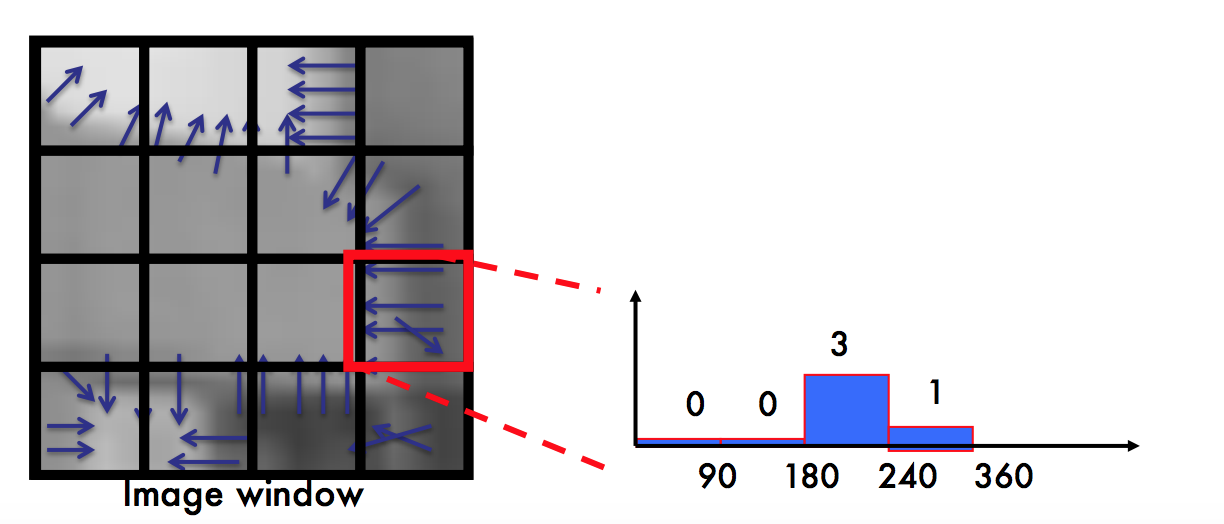
\includegraphics[width=0.5\textwidth]{sift_bins}
\end{figure}

\item Weight the set of histograms by a Gaussian around the center of the keypoint; use $\sigma$ that is half the scale of the keypoint. 

\begin{figure}[h]
\centering
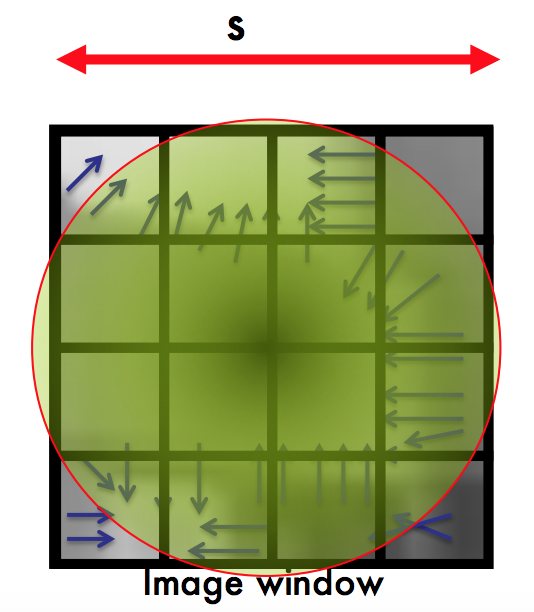
\includegraphics[width=0.25\textwidth]{sift_gblur}
\end{figure}

\item Concatenate these weighted histograms $h_i$ for $i = 1, ..., N^2$ to form a $1 \times MN^2$ vector H. 
\item Normalize the feature descriptor H. 
\end{enumerate}

\noindent Typically, and in the original paper, M = 8, N = 4 for a 128 dimensional descriptor H. 


\subsubsection{Matching SIFT Keypoints}
The procedure for matching SIFT keypoints in order to reconstruct bounding boxes is left as a homework exercise. Overall, the SIFT descriptor is a significant upgrade to the patch descriptor. 

\subsection{HoG}
The Histogram of oriented Gradients descriptor is a variant of SIFT that initially showed state of the art accuracy on pedestrian detection when published by Triggs and Dalal, 2005. In HoG, histograms are sampled on a dense regular grid around the object (unlike the use of DoG in SIFT), and gradients are contrast normalized in overlapping blocks. An implementation of the HoG descriptor is left as an exercise for homework. 

\begin{figure}
\centering
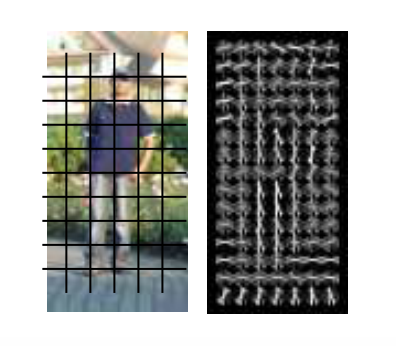
\includegraphics[width=0.5\textwidth]{hog}
\caption{The HoG descriptor applied to pedestrians.}
\end{figure}

\subsection{Shape Context}

The shape context descriptor is based on the following premise: we compute how many other keypoints fall into a bin of a specific distance and orientation relative to a specific keypoint. This allows a comparison of shape because the descriptor compares the relative position of keypoints. 

\begin{figure}[h]
\centering
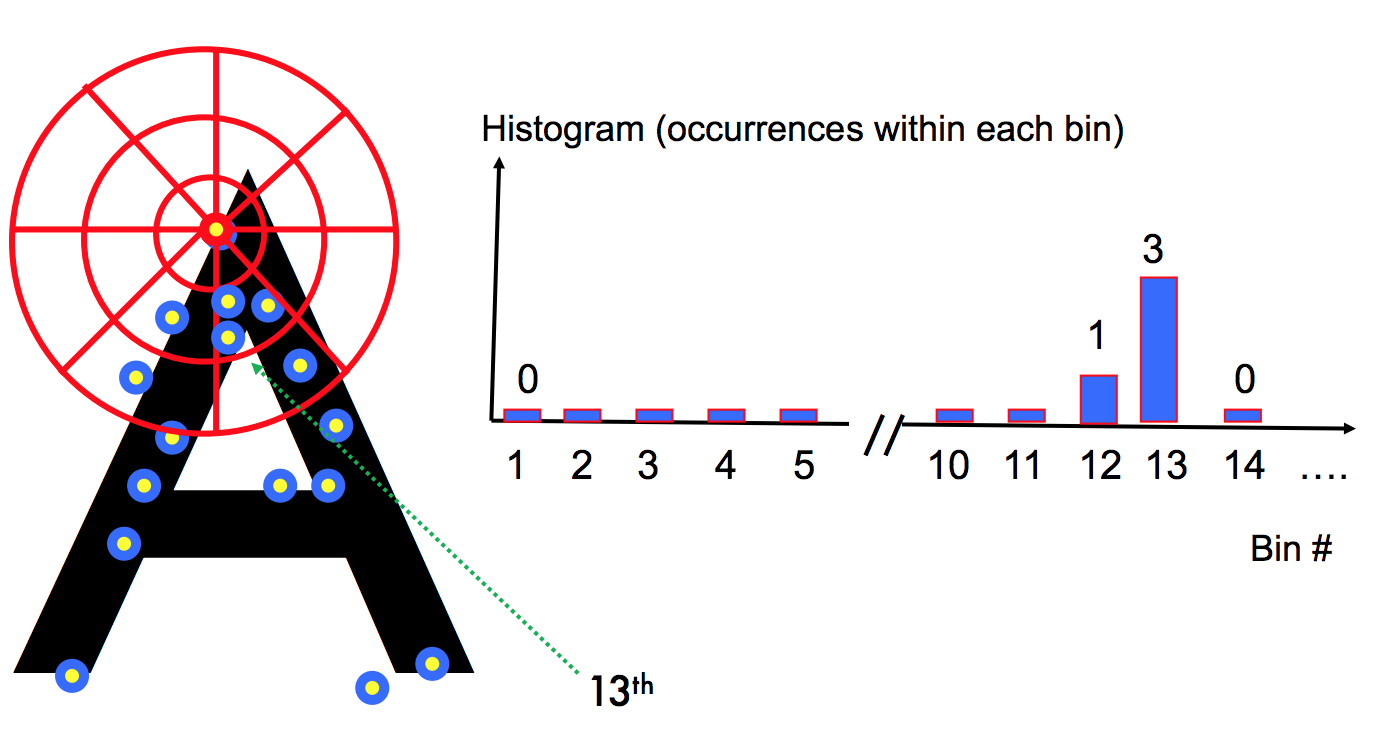
\includegraphics[width=0.5\textwidth]{shape_desc}
\caption{The shape descriptor applied to the letter A. All dots correspond to keypoints, and the sections of the red circle correspond to different bins.}
\end{figure}

\end{document}